\chapter{Nonlinear Filtering}
\label{ch:nonlinear}

\begin{objectives}
\begin{itemize}
  \item Derive the extended Kalman filter by linearization, and identify every approximation it makes.
  \item Understand the iterated EKF as Gauss--Newton.
  \item Understand the unscented transform and the unscented Kalman filter.
  \item Understand particle filters and why they do not scale to VIO.
  \item Know why VIO filters are EKFs, and what that implies for how they must be designed.
\end{itemize}
\end{objectives}

Real systems are nonlinear: rotations enter through trigonometric functions, projections divide by depth. A Gaussian pushed through a
nonlinear function is no longer Gaussian (\cref{sec:linearization}), so the exact Bayes filter of \cref{ch:kf} no longer has a finite-dimensional
form. This chapter presents the three main families of approximations. The extended Kalman filter, the basis of this project, is treated in
detail; the others are presented so that the choice is understood.

% ==============================================================================
\section{The extended Kalman filter}

\subsection{The model}

A nonlinear discrete-time model reads
\begin{equation}
  x_k = f(x_{k-1}, u_k, w_k), \qquad z_k = h(x_k) + n_k,
  \label{eq:nonlinear-model}
\end{equation}
with known input $u_k$ (an IMU reading, for instance), process noise $w_k \sim \N(0, Q_k)$ and measurement noise $n_k \sim \N(0, R_k)$.

\subsection{Derivation}

The \term{extended Kalman filter} (EKF) applies the Kalman filter to a linearization of the model about the current estimate.

\paragraph{Prediction.} Expand $f$ to first order around the previous estimate and zero noise:
\begin{equation}
  x_k \approx f(\hat x_{k-1}^+, u_k, 0) + F_k\,(x_{k-1} - \hat x_{k-1}^+) + L_kw_k,
  \qquad F_k = \frac{\partial f}{\partial x}\Big|_{\hat x_{k-1}^+},\quad L_k = \frac{\partial f}{\partial w}\Big|_{\hat x_{k-1}^+} .
\end{equation}
Taking the mean and covariance of the right-hand side (\cref{prop:affine}):
\begin{equation}
  \hat x_k^- = f(\hat x_{k-1}^+, u_k, 0), \qquad P_k^- = F_kP_{k-1}^+F_k\T + L_kQ_kL_k\T .
\end{equation}
The mean is propagated through the \emph{nonlinear} function, the covariance through its Jacobian.

\paragraph{Update.} Expand $h$ around the prediction, $h(x_k) \approx h(\hat x_k^-) + H_k(x_k - \hat x_k^-)$ with $H_k = \partial h/\partial x|_{\hat x_k^-}$, and apply the linear update with
the innovation computed from the nonlinear prediction:
\begin{equation}
\begin{gathered}
  r_k = z_k - h(\hat x_k^-), \qquad S_k = H_kP_k^-H_k\T + R_k, \qquad K_k = P_k^-H_k\T S_k\inv, \\
  \hat x_k^+ = \hat x_k^- + K_kr_k, \qquad P_k^+ = (I - K_kH_k)P_k^-(I - K_kH_k)\T + K_kR_kK_k\T .
\end{gathered}
\end{equation}

\subsection{What the EKF gets wrong}

Every step above is exact for linear models. For nonlinear models the EKF makes three approximations:
\begin{enumerate}
  \item \emph{Gaussianity}: the true prior and posterior are not Gaussian, but are represented by a mean and a covariance.
  \item \emph{Mean bias}: the predicted mean is $f(\hat x)$, not $\E[f(x)]$. By \cref{sec:linearization} the difference is about
        $\tfrac12\sum_ie_i\tr(\nabla^2f_i\,P)$, proportional to the curvature times the covariance.
  \item \emph{Covariance error}: $FPF\T$ ignores higher-order terms, and the Jacobians are evaluated at the \emph{estimate}, not at the unknown true state.
\end{enumerate}
All three errors grow with the size of the uncertainty relative to the scale over which the functions curve. When errors are small, the EKF is
excellent; when they are large, it can be badly wrong, and in particular it can become \emph{inconsistent}: report a covariance smaller than its
actual errors. The third approximation has a subtle long-term consequence in VIO, a spurious gain of information about unobservable directions
(\cref{ch:observability}).

\subsection{The iterated EKF}

By \cref{prop:ekf-gn}, the EKF update is one Gauss--Newton step on the MAP cost $\tfrac12\|x - \hat x^-\|^2_{(P^-)\inv} + \tfrac12\|z - h(x)\|^2_{R\inv}$, linearized at the prior
mean. When the measurement function is strongly nonlinear, that single step can be inaccurate. The \term{iterated EKF} (IEKF) repeats it,
re-linearizing at the latest iterate $x^{(i)}$ while keeping the prior term:
\begin{equation}
  x^{(i+1)} = \hat x^- + K^{(i)}\big(z - h(x^{(i)}) - H^{(i)}(\hat x^- - x^{(i)})\big), \qquad K^{(i)} = P^-H^{(i)\T}\big(H^{(i)}P^-H^{(i)\T} + R\big)\inv,
\end{equation}
with $H^{(i)}$ evaluated at $x^{(i)}$ and $x^{(0)} = \hat x^-$. The first iteration is the EKF. The covariance is computed with the last Jacobian. Iteration
helps when the measurement is very informative relative to the prior, so that the posterior lies far from the prior mean, where the first
linearization is poor.

% ==============================================================================
\section{Sigma-point filters}

\subsection{The unscented transform}

Linearization approximates the \emph{function}. The \term{unscented transform} approximates the \emph{distribution} instead, by a small set of
deterministically chosen \emph{sigma points} that have the right mean and covariance, and pushes each point through the exact nonlinear function.

For $x \in \R^n$ with mean $\mu$ and covariance $P = LL\T$ (Cholesky), choose $\lambda = \alpha^2(n + \kappa) - n$ and the $2n + 1$ points
\begin{equation}
  \chi_0 = \mu, \qquad \chi_i = \mu + \sqrt{n + \lambda}\,\ell_i, \qquad \chi_{n+i} = \mu - \sqrt{n + \lambda}\,\ell_i, \qquad i = 1, \dots, n,
\end{equation}
where $\ell_i$ is the $i$-th column of $L$, with weights
\begin{equation}
  W_0^{(m)} = \frac{\lambda}{n + \lambda}, \quad W_0^{(c)} = \frac{\lambda}{n + \lambda} + (1 - \alpha^2 + \beta), \quad W_i^{(m)} = W_i^{(c)} = \frac{1}{2(n + \lambda)} .
\end{equation}
Propagate $\gamma_i = f(\chi_i)$ and recombine:
\begin{equation}
  \bar y = \sum_iW_i^{(m)}\gamma_i, \qquad P_y = \sum_iW_i^{(c)}(\gamma_i - \bar y)(\gamma_i - \bar y)\T .
\end{equation}
The points are placed symmetrically along the principal axes of the uncertainty, so the weighted points reproduce $\mu$ and $P$ exactly. Expanding $f$
in a Taylor series about $\mu$ shows that $\bar y$ captures the second-order (curvature) term of the mean that linearization misses, and that
$P_y$ is correct to second order, without computing any derivatives. The parameters $\alpha$, $\beta$, $\kappa$ control the spread of the points
($\beta = 2$ is optimal for Gaussians).

\begin{figure}[t]
  \centering
  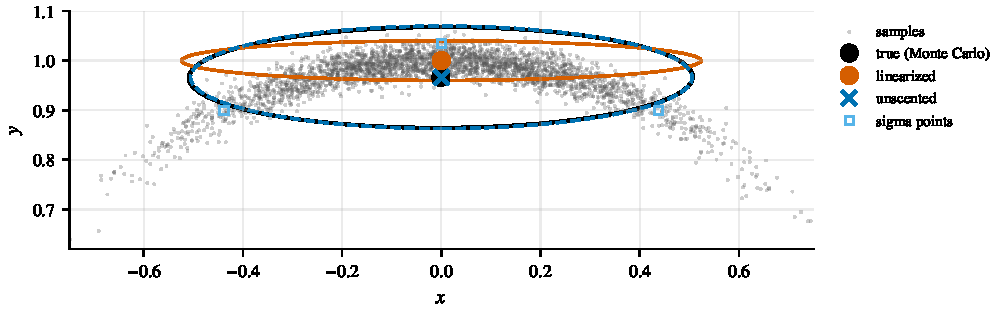
\includegraphics[width=\textwidth]{fig_ut.pdf}
  \caption{A range-bearing measurement converted to Cartesian coordinates, with $\sigma_r = 0.02$ and $\sigma_\phi = 15^\circ$. Monte Carlo samples of the true
  distribution (dots), its true mean and covariance (black), the linearized approximation (orange), and the unscented transform (blue, dashed), with the five
  sigma points; ellipses are $2\sigma$. Linearization places the mean on the circle, where it should not be; the unscented transform recovers the inward shift of the
  mean and a better covariance.}
  \label{fig:ut}
\end{figure}

\subsection{The unscented Kalman filter}

The \emph{unscented Kalman filter} (UKF) uses the unscented transform for both steps. Prediction: generate sigma points from $(\hat x^+, P^+)$, propagate them
through $f$, and recombine into $(\hat x^-, P^-)$, adding $Q$. Update: generate sigma points from $(\hat x^-, P^-)$, push them through $h$ to get the predicted
measurement $\bar z$ and its covariance $S$ (adding $R$), and the cross-covariance $P_{xz} = \sum_iW_i^{(c)}(\chi_i - \hat x^-)(\gamma_i - \bar z)\T$; then
$K = P_{xz}S\inv$, $\hat x^+ = \hat x^- + K(z - \bar z)$ and $P^+ = P^- - KSK\T$. These are the LMMSE formulas of \cref{thm:lmmse} with moments estimated by the
sigma points rather than by linearization. On manifolds, sigma points are generated in the tangent space and mapped with $\bplus$, and their mean is
computed iteratively as in \cref{ch:lie}.

The UKF costs about $2n + 1$ evaluations of $f$ and $h$ per step instead of Jacobians, which is attractive when Jacobians are hard to derive. For VIO
with a 75-dimensional state, the $151$ propagations of the full state per IMU sample are expensive, and the accuracy gain over a well-designed
error-state EKF is small, because the error-state formulation already keeps the nonlinearity mild.

% ==============================================================================
\section{Particle filters}

A \term{particle filter} represents the posterior by $N$ weighted samples (particles) $\{x^{(j)}, w^{(j)}\}$, which can represent any distribution,
multi-modal ones included. The basic \emph{sequential importance resampling} (SIR) algorithm:
\begin{enumerate}
  \item \emph{Predict}: move each particle through the dynamics with a random noise sample, $x_k^{(j)} = f(x_{k-1}^{(j)}, u_k, w^{(j)})$.
  \item \emph{Weight}: multiply each weight by the likelihood of the measurement, $w^{(j)} \gets w^{(j)}p(z_k\mid x_k^{(j)})$, and normalize.
  \item \emph{Resample}: when the effective sample size $N_{\mathrm{eff}} = 1/\sum_j(w^{(j)})^2$ falls too low, draw $N$ new particles with probabilities $w^{(j)}$ and
        reset the weights to $1/N$, so that particles concentrate where the posterior mass is.
\end{enumerate}
Particle filters are exact as $N\to\infty$ and excel at low-dimensional problems with multi-modal posteriors, such as localizing a robot in a known
map. Their weakness is dimension: the number of particles needed to cover a distribution grows roughly exponentially with the state dimension.
For the 15 to 75 dimensions of VIO they are impractical, except in hybrid forms that sample only a few variables.

% ==============================================================================
\section{Why VIO uses the EKF}

\begin{center}\small
\begin{tabularx}{\textwidth}{@{}>{\raggedright\arraybackslash}p{0.2\textwidth}>{\raggedright\arraybackslash}X>{\raggedright\arraybackslash}X>{\raggedright\arraybackslash}X@{}}
\toprule
 & EKF & UKF & particle filter \\
\midrule
cost per step & Jacobians, $\mathcal{O}(n^3)$ & $2n + 1$ propagations, $\mathcal{O}(n^3)$ & $N$ propagations, $N$ huge for large $n$ \\
derivatives needed & yes & no & no \\
non-Gaussian posteriors & no & no & yes \\
accuracy for small errors & excellent & excellent & good (noisy) \\
used in VIO & MSCKF, OpenVINS, ROVIO (iterated) & rarely & no \\
\bottomrule
\end{tabularx}
\end{center}

Visual-inertial odometry has a high-dimensional state, a fast prediction rate (hundreds of Hz), and uncertainties that, once the filter is initialized,
are small compared with the curvature of its models. Those are exactly the conditions under which the EKF is accurate and the alternatives are
expensive. The design principle that makes this work is to keep the linearized errors small: estimate the \emph{error} of a nominal state that
absorbs the large nonlinear motion, and reset it after every correction. That is the error-state Kalman filter of the next chapter.

\begin{takeaways}
\begin{itemize}
  \item The EKF propagates the mean through the nonlinear model and the covariance through its Jacobians, evaluated at the estimate.
  \item Its errors (non-Gaussianity, mean bias, covariance error, estimate-dependent Jacobians) grow with uncertainty relative to curvature.
  \item The iterated EKF is Gauss--Newton on the MAP cost; it helps when measurements are very informative.
  \item The unscented transform propagates sigma points through the exact function and captures second-order effects without derivatives.
  \item Particle filters handle any distribution but scale exponentially with dimension.
  \item VIO uses EKFs with small, frequently reset errors: the error-state formulation.
\end{itemize}
\end{takeaways}

\begin{exercises}
  \item Write the EKF for a planar robot with state $(x, y, \psi)$ driven by speed and turn rate and measured by range to a known beacon. Identify where
        linearization error enters.
  \item Reproduce \cref{fig:ut}. Increase $\sigma_\phi$ until the linearized mean lies outside the $1\sigma$ ellipse of the true distribution.
  \item Show that the unscented transform reproduces the mean and covariance exactly for a linear function.
  \item Show that for a scalar $x \sim \N(\mu, \sigma^2)$ and $f(x) = x^2$, the unscented transform with $n = 1$, $\kappa = 2$, $\alpha = 1$ gives the exact mean $\mu^2 + \sigma^2$.
  \item Implement a particle filter for a 1D robot localizing itself from range measurements to two landmarks, and observe a bimodal posterior.
\end{exercises}
% Solutions to the exercises of Chapter 13.
\begin{solutions}
  \item State $x = (p_x, p_y, \psi)$, inputs $(v, \omega)$ with noise $(n_v, n_\omega)$, beacon at $b = (b_x, b_y)$ with known position.
        \begin{itemize}[leftmargin=1.2em]
          \item \emph{Prediction}: $f(x) = \big(p_x + v\Dt\cos\psi,\ p_y + v\Dt\sin\psi,\ \psi + \omega\Dt\big)$, with Jacobians
                \[
                  F = \begin{bmatrix}1 & 0 & -v\Dt\sin\hat\psi\\ 0 & 1 & v\Dt\cos\hat\psi\\ 0 & 0 & 1\end{bmatrix}, \qquad
                  L = \begin{bmatrix}\Dt\cos\hat\psi & 0\\ \Dt\sin\hat\psi & 0\\ 0 & \Dt\end{bmatrix},
                \]
                and $P^- = FPF\T + L\diag(\sigma_v^2, \sigma_\omega^2)L\T$.
          \item \emph{Update}: $h(x) = \rho = \|p - b\|$, $H = \big[(\hat p_x - b_x)/\hat\rho,\ (\hat p_y - b_y)/\hat\rho,\ 0\big]$, then the standard update.
        \end{itemize}
        Linearization error enters in three places. (i) In the prediction through $\cos\psi$ and $\sin\psi$: with a large heading uncertainty the predicted
        positions spread along an arc, the banana of \cref{fig:banana}, which $FPF\T$ approximates by an ellipse. (ii) In the update through the curvature of the
        range: $\nabla^2h$ has the eigenvalue $1/\rho$ in the direction perpendicular to the line of sight, so the neglected second-order term is about
        $\sigma_\perp^2/(2\rho)$, harmless far from the beacon and large close to it (and $H$ is undefined at $\rho = 0$). (iii) In the heading: the range does not
        depend on $\psi$ ($H_\psi = 0$), so the heading is corrected only through the position-heading correlation that motion builds in $P$, which is
        itself a linearized quantity. When the heading error is large, those correlations are wrong and the corrections are too.

  \item With the figure's $\sigma_r = 0.02$, the true distribution of $(x, y) = (r\cos\phi, r\sin\phi)$ for $\phi \sim \N(\pi/2, \sigma_\phi^2)$ has mean $(0, e^{-\sigma_\phi^2/2})$ and
        $\Var(y) = (1 + \sigma_r^2)(1 + e^{-2\sigma_\phi^2})/2 - e^{-\sigma_\phi^2}$, while linearization predicts the mean $(0, 1)$. The covariance is diagonal by symmetry,
        so the Mahalanobis distance of the linearized mean is $d = (1 - e^{-\sigma_\phi^2/2})/\sqrt{\Var(y)}$:
        \begin{center}\small
        \begin{tabular}{@{}l c c c c c c@{}}
        \toprule
        $\sigma_\phi$ & $15^\circ$ & $30^\circ$ & $45^\circ$ & $60^\circ$ & $75^\circ$ & $90^\circ$ \\
        \midrule
        $d$ & 0.67 & 0.75 & 0.81 & 0.90 & 0.99 & 1.10 \\
        \bottomrule
        \end{tabular}
        \end{center}
        The linearized mean leaves the $1\sigma$ ellipse at $\sigma_\phi \approx 76^\circ$ (confirmed by Monte Carlo). Notice that it never gets very far: in the
        small-angle regime $d^2 \approx (\sigma_\phi^4/4)/(\sigma_r^2 + \sigma_\phi^4/2) < \tfrac12$, because the true distribution spreads along the arc as fast as its mean moves
        inward. The more telling failure is the shape: the true distribution is a thin curved arc, and the linearized ellipse puts most of its
        probability where the true one has none.

  \item For $f(x) = Ax + b$ the transformed sigma points are $y_0 = A\mu + b$ and $y_{i}, y_{n+i} = A\mu + b \pm\sqrt{n + \lambda}\,A\ell_i$. The mean weights sum to
        one ($\frac{\lambda}{n + \lambda} + \frac{2n}{2(n + \lambda)} = 1$) and the $\pm$ pairs cancel, so $\bar y = \sum_iW_i^{(m)}y_i = A\mu + b$. In the covariance the central point
        contributes nothing ($y_0 - \bar y = 0$, so the value of $W_0^{(c)}$ and of $\beta$ is irrelevant), and each pair contributes
        $2\cdot\frac{1}{2(n + \lambda)}(n + \lambda)A\ell_i\ell_i\T A\T$:
        \[
          \sum_iW_i^{(c)}(y_i - \bar y)(y_i - \bar y)\T = A\Big(\sum_{i=1}^n\ell_i\ell_i\T\Big)A\T = ALL\T A\T = APA\T .
        \]
        The unscented transform is exact for linear functions, as it must be to be consistent with the Kalman filter.

  \item With $n = 1$, $\kappa = 2$ and $\alpha = 1$: $\lambda = 1\cdot3 - 1 = 2$, $n + \lambda = 3$, sigma points $\mu$ and $\mu \pm \sqrt3\,\sigma$, weights $W_0^{(m)} = \tfrac23$ and
        $W_{1,2}^{(m)} = \tfrac16$. For $f(x) = x^2$,
        \[
          \tfrac23\mu^2 + \tfrac16\big((\mu + \sqrt3\sigma)^2 + (\mu - \sqrt3\sigma)^2\big) = \tfrac23\mu^2 + \tfrac16\big(2\mu^2 + 6\sigma^2\big) = \mu^2 + \sigma^2 = \E[x^2],
        \]
        exactly, whereas linearization gives $\mu^2$. (The choice $\kappa = 3 - n$ also makes the sigma points reproduce the fourth moment $3\sigma^4$ of a scalar
        Gaussian: $\tfrac16\cdot2\cdot9\sigma^4 = 3\sigma^4$.)

  \item A simple model that produces bimodality: landmarks at $0$ and $10$ on a line, and a sensor that reports the range to the \emph{nearest} landmark
        without saying which one it is ($z = \min(|x|, |x - 10|) + n$, $\sigma_z = 0.1$). The robot starts at $x = 2$ with a uniform prior on $[0, 10]$ and
        then moves right by $0.5$ per step (odometry noise $0.05$). A bootstrap particle filter with 2000 particles: propagate each particle with the
        odometry plus sampled noise, multiply its weight by the likelihood $\exp(-(z - h(x_i))^2/2\sigma_z^2)$, normalize, and resample when the effective
        sample size $1/\sum_iw_i^2$ drops below $N/2$. After the first measurement ($z = 1.87$) the posterior has two equal modes, near $1.9$ and near $8.1$
        (weights $0.52$ and $0.48$), symmetric about $5$; its mean, $4.9$, is a place where the robot certainly is not, which is what a Gaussian filter
        would report. After the first move the mirror hypothesis predicts a range of about $1.4$ (it approaches the landmark at 10) while the
        measurement says $2.3$; its weight drops to zero and the filter tracks the true position from then on. A Kalman-type filter cannot represent
        the bimodal stage at all: it would either lock onto one mode, possibly the wrong one, or average them.
\end{solutions}

